%% LyX 2.4.4 created this file.  For more info, see https://www.lyx.org/.
%% Do not edit unless you really know what you are doing.
\documentclass[english]{article}
\usepackage[T1]{fontenc}
\usepackage[latin9]{inputenc}
\usepackage{enumitem}
\usepackage{amsmath}
\usepackage{amsthm}
\usepackage{cancel}
\usepackage{geometry}
\geometry{verbose,tmargin=1in,bmargin=1in,lmargin=1in,rmargin=1in}

\makeatletter

%%%%%%%%%%%%%%%%%%%%%%%%%%%%%% LyX specific LaTeX commands.
%% Because html converters don't know tabularnewline
\providecommand{\tabularnewline}{\\}

%%%%%%%%%%%%%%%%%%%%%%%%%%%%%% Textclass specific LaTeX commands.
\numberwithin{equation}{section}
\numberwithin{figure}{section}
\newlength{\lyxlabelwidth}      % auxiliary length 

%%%%%%%%%%%%%%%%%%%%%%%%%%%%%% User specified LaTeX commands.
\usepackage{fancyhdr}
\usepackage{lastpage}
\pagestyle{fancy}
\usepackage{enumitem}
\usepackage{ifthen}
%sets math fonts to be more readable
\everymath=\expandafter{\the\everymath\displaystyle}
%\DeclareMathSizes{10}{10}{10}{10}
\usepackage{multicol}

\usepackage{tikz}
\usetikzlibrary{plotmarks}
\usepackage{pgfplots}
\pgfplotsset{compat=newest}

\usepackage{calc}
\usepackage[nomessages]{fp}

\usepackage{advdate}    % Advancing/saving dates
\usepackage{datetime}   % Dates formatting
\usepackage{datenumber} % Counters for dates
% Added by lyx2lyx
\setlength{\parskip}{\smallskipamount}
\setlength{\parindent}{0pt}

\makeatother

\usepackage{babel}
\begin{document}
\renewcommand{\author}{Dr.\,James Ashe}

\newcommand{\classNum}{107}

\newcommand{\classSec}{7 and 10}

\newcommand{\nameType}{\hspace{2cm}Name:}

\newcommand{\examType}{Quiz 2: 1.1 \& 1.2}

\renewcommand{\date}{\formatdate{15}{9}{2014}}

%%First page's header%%%%%%%%%%%%%%%%%%%%%%
\fancypagestyle{firststyle} %%header settings for first pagr
{
	\fancyhead[L]{MTH \classNum{}(\classSec{}) \author{}\\
	\textbf{\examType{}} \date{}}
	\fancyhead[C]{\textbf{\nameType}}
	\setlength{\headsep}{14pt}
}
%%%%%%%%%%%%%%%%%%%%%%%%%%%%%%%%%%%%%%%%%%

%%Next page's header%%%%%%%%%%%%%%%%%%%%%%%
%\setlist{nolistsep}
\lhead{MTH \classNum{}(\classSec{})} 
\chead{\textbf{\nameType}} 
\cfoot{\thepage{}~of~\pageref{LastPage}} 
\setlength{\headsep}{5pt} 
%%%%%%%%%%%%%%%%%%%%%%%%%%%%%%%%%%%%%%%%%%%

%%Various settings; see the preamble for other settings%%%%%
%%\setenumerate[0]{leftmargin=12pt,itemindent=0pt,labelwidth=0pt}
\renewcommand{\labelenumi}{\textbf{\arabic{enumi}.}}
\renewcommand{\labelenumii}{\textbf{\alph{enumii}.}}
\thispagestyle{firststyle}
%%%%%%%%%%%%%%%%%%%%%%%%%%%%%%%%%%%%%%%%%%
\newcommand{\xmax}{10}
\newcommand{\xmin}{-10}
\newcommand{\xstep}{0} %must be xmin+n
\newcommand{\ymax}{10}
\newcommand{\ymin}{-10}
\newcommand{\ystep}{0} %must be ymin+n

\newcommand{\xspace}{\vspace{.75cm}}

\emph{You must show work to receive credit. Unless indicated otherwise,
each problem is worth equal value.}
\begin{enumerate}[resume]
\item Construct a Venn diagram to determine the validity of the given argument.

\begin{enumerate}
\item \vspace{-25pt} \begin{multicols}{2}%
\begin{tabular}{l}
\tabularnewline
\tabularnewline
1. All homeless people are unemployed.\tabularnewline
2. Bill Gates is not unemployed.\tabularnewline
\hline 
Therefore, Bill Gates is not homeless\tabularnewline
\textbf{$\Rightarrow$Valid}\tabularnewline
\end{tabular}\columnbreak\\
\vfill%%%%little circle in big%%%%%
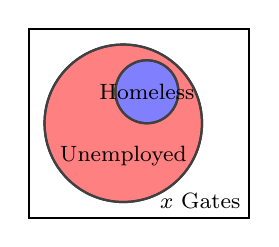
\begin{tikzpicture}[scale=.4]
	\def\circleA{(1,-1) circle (2.5)} %A
	\def\circleB{(0:1.75) circle (1)} %B

	\colorlet{circle edgeA}{black!75} 
	\colorlet{circle areaA}{red!50}
	\colorlet{circle edgeB}{black!75} 
	\colorlet{circle areaB}{blue!50}

	\tikzset{
		filledA/.style={fill=circle areaA, draw=circle edgeA, thick},
		filledB/.style={fill=circle areaB, draw=circle edgeB, thick},
		outlineA/.style={draw=circle edgeA, thick},
		outlineB/.style={draw=circle edgeB, thick},
	}

	\begin{scope}[fill opacity=1.0]         
			\fill[filledA] \circleA;
			\fill[filledB] \circleB;    
	\end{scope}
	
	\footnotesize
	\draw[outlineA] \circleA node[below = 5pt] {Unemployed} node[below = 10pt] {$$}; 
	\draw[outlineB] \circleB node {Homeless} node[below = 5pt] {$$};
	%\node[anchor=south] at (current bounding box.north) {$A \cup B$}; 
	\draw[thick] (-2,-4) rectangle (5,2) node[anchor=south east] at (current bounding box.south east) {$x$ Gates};
	%\draw \circleA node[below=30pt,right=0pt] {\footnotesize{\emph{Gates}}};
\end{tikzpicture} 

\end{multicols}
\item \vspace{-25pt} \begin{multicols}{2}%
\begin{tabular}{l}
\tabularnewline
\tabularnewline
1. No vegetarian owns a gun.\tabularnewline
2. All policemen own guns.\tabularnewline
\hline 
Therefore, no policeman is a vegetarian.\tabularnewline
\textbf{$\Rightarrow$Valid}\tabularnewline
\end{tabular}\columnbreak\\
\vfill%%%%little circle in big%%%%%
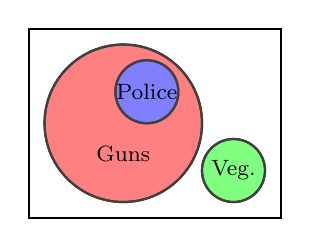
\begin{tikzpicture}[scale=.4]
	\def\circleA{(1,-1) circle (2.5)} %A
	\def\circleB{(0:1.75) circle (1)} %B
	\def\circleC{(4.5,-2.5) circle (1)} %C


	\colorlet{circle edgeA}{black!75} 
	\colorlet{circle areaA}{red!50}
	\colorlet{circle edgeB}{black!75} 
	\colorlet{circle areaB}{blue!50}
	\colorlet{circle edgeC}{black!75} 
	\colorlet{circle areaC}{green!50}

	\tikzset{
		filledA/.style={fill=circle areaA, draw=circle edgeA, thick},
		filledB/.style={fill=circle areaB, draw=circle edgeB, thick},
		filledC/.style={fill=circle areaC, draw=circle edgeC, thick},
		outlineA/.style={draw=circle edgeA, thick},
		outlineB/.style={draw=circle edgeB, thick},
		outlineC/.style={draw=circle edgeC, thick}
	}

	\begin{scope}[fill opacity=1.0]         
			\fill[filledA] \circleA;
			\fill[filledB] \circleB;
			\fill[filledC] \circleC;  
	\end{scope}
	
	\footnotesize
	\draw[outlineA] \circleA node[below = 5pt] {Guns} node[below = 10pt] {$$}; 
	\draw[outlineB] \circleB node {Police} node[below = 5pt] {$$};
	\draw[outlineC] \circleC node {Veg.} node[below = 5pt] {$$};
	%\node[anchor=south] at (current bounding box.north) {$A \cup B$}; 
	\draw[thick] (-2,-4) rectangle (6,2) node[anchor=south east] at (current bounding box.south east) {$$};
	%\draw \circleA node[below=30pt,right=0pt] {\footnotesize{\emph{Gates}}};
\end{tikzpicture} 

\end{multicols}
\item \vspace{-25pt} \begin{multicols}{2}%
\begin{tabular}{l}
\tabularnewline
\tabularnewline
1. No professor is a millionaire.\tabularnewline
2. No millionaire is illiterate.\tabularnewline
\hline 
Therefore, no professor is illiterate.\tabularnewline
$\mbox{\ensuremath{\Rightarrow}}$\textbf{Invalid}\tabularnewline
\end{tabular}\columnbreak\\
\vfill%%%%little circle in big%%%%%
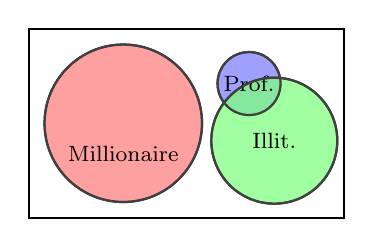
\begin{tikzpicture}[scale=.4]
	\def\circleA{(1,-1) circle (2.5)} %A
	\def\circleB{(3:5) circle (1)} %B
	\def\circleC{(-15:6) circle (2)} %C


	\colorlet{circle edgeA}{black!75} 
	\colorlet{circle areaA}{red!50}
	\colorlet{circle edgeB}{black!75} 
	\colorlet{circle areaB}{blue!50}
	\colorlet{circle edgeC}{black!75} 
	\colorlet{circle areaC}{green!50}

	\tikzset{
		filledA/.style={fill=circle areaA, draw=circle edgeA, thick},
		filledB/.style={fill=circle areaB, draw=circle edgeB, thick},
		filledC/.style={fill=circle areaC, draw=circle edgeC, thick},
		outlineA/.style={draw=circle edgeA, thick},
		outlineB/.style={draw=circle edgeB, thick},
		outlineC/.style={draw=circle edgeC, thick}
	}

	\begin{scope}[fill opacity=.75]         
			\fill[filledA] \circleA;
			\fill[filledB] \circleB;
			\fill[filledC] \circleC;  
	\end{scope}
	
	\footnotesize
	\draw[outlineA] \circleA node[below = 5pt] {Millionaire} node[below = 10pt] {$$}; 
	\draw[outlineB] \circleB node {Prof.} node[below = 5pt] {$$};
	\draw[outlineC] \circleC node {Illit.} node[below = 5pt] {$$};
	%\node[anchor=south] at (current bounding box.north) {$A \cup B$}; 
	\draw[thick] (-2,-4) rectangle (8,2) node[anchor=south east] at (current bounding box.south east) {$$};
	%\draw \circleA node[below=30pt,right=0pt] {\footnotesize{\emph{Gates}}};
\end{tikzpicture} 

\end{multicols} \vfill
\end{enumerate}
\end{enumerate}
\begin{enumerate}
\item Which of the following are statements? Why or why not?

\begin{enumerate}
\item $3+7=9$

\begin{enumerate}
\item []Yes, read ``three plus seven is equal to nine'', and this is
either true or false.
\end{enumerate}
\item Solve the equation $3+7=x$.

\begin{enumerate}
\item []No, it is a command. Commands are neither true nor false.
\end{enumerate}
\item Is $\sqrt{2}$ an irrational number?

\begin{enumerate}
\item []No, it is a question. Questions are neither true nor false.\vfill
\end{enumerate}
\end{enumerate}
\item Write a sentence that negates the statement.

\begin{enumerate}
\item Some cats have three legs.

\begin{enumerate}
\item []No cat has three legs.
\end{enumerate}
\item No cat has three legs. 

\begin{enumerate}
\item []Some cats have three legs.
\end{enumerate}
\item All of the cats have three legs.

\begin{enumerate}
\item []Some cats do not have three legs.
\end{enumerate}
\item The cat is not blue.

\begin{enumerate}
\item []The cat is blue.\vfill
\end{enumerate}
\end{enumerate}
\item Translate the sentence into symbolic form.

\begin{enumerate}
\item It is a square and a rectangle. 

\begin{enumerate}
\item []$s\wedge r$
\end{enumerate}
\item If John is male then he is human.

\begin{enumerate}
\item []$m\rightarrow h$
\end{enumerate}
\item All squares are rectangles.

\begin{enumerate}
\item []$s\rightarrow r$
\end{enumerate}
\item All whole numbers are even or odd.

\begin{enumerate}
\item []$w\rightarrow(e\vee o)$
\end{enumerate}
\item No square is a triangle.

\begin{enumerate}
\item []$s\rightarrow\sim t$
\end{enumerate}
\item Being an orthodontist is sufficient for being a dentist.

\begin{enumerate}
\item []$o\rightarrow d$
\end{enumerate}
\item Not being a monkey is necessary for being an ape.

\begin{enumerate}
\item []$a\rightarrow\sim m$\vfill
\end{enumerate}
\end{enumerate}
\item Using the symbolic representations

\begin{itemize}
\item []$p$: The car costs $\$70,000$.
\item []$q$: The car goes $140$ mph.
\item []$r$: the car is red.
\end{itemize}
express the following compound statements in symbolic form.
\begin{enumerate}
\item All red cars go $140$ mph.

\begin{enumerate}
\item []$r\rightarrow q$
\end{enumerate}
\item The car is red, goes $140$ mph, and does not cost $\$70,000$.

\begin{enumerate}
\item []$r\wedge q\wedge\sim p$
\end{enumerate}
\item If the car does not cost $\$70,000$, it does not go $140$ mph.

\begin{enumerate}
\item []$\sim p\rightarrow\sim q$
\end{enumerate}
\item The car is red, and it does not cost $\$70,000$ or go $140$ mph.

\begin{enumerate}
\item []$r\wedge\sim(p\vee q)$
\end{enumerate}
\item Being able to go $140$ mph is sufficient for a car to cost $\$70,000$
or be red.

\begin{enumerate}
\item []$q\rightarrow(p\vee r)$
\end{enumerate}
\item Not being red is necessary for a car to cost $\$70,000$ and not go
$140$ mph.

\begin{enumerate}
\item []$(p\wedge\sim q)\rightarrow\sim r$\vfill
\end{enumerate}
\end{enumerate}
\end{enumerate}

\end{document}
